\documentclass{article}
\usepackage[utf8]{inputenc}
\usepackage{graphicx}
\usepackage{tabularx}
\usepackage{booktabs}
\usepackage{hyperref}
\usepackage{listings}
\usepackage[margin=0.85in]{geometry}
\usepackage[backend=bibtex,style=ieee]{biblatex}
\addbibresource{textmining_julki092.bib}
\newcommand{\HRule}[1]{\rule{\linewidth}{#1}}

\begin{document}
	
	\title{\textsc{732A92 Text Mining} \\ [2.0cm]
		\HRule{0.5pt} \\
		\LARGE \textbf{\uppercase{Classifying Stock Price Movements based on 8-K SEC filings}}
		\HRule{2pt} \\ [0.5cm]
		\normalsize \today \vspace*{5\baselineskip}}
	
	\date{}
	
	\author{
		Name: Julius Kittler \\ 
		Student ID: julki092 \\ 
		Link\"{o}ping University}
	
	\maketitle
	\newpage
	
	\begin{abstract}
		
		For over a century, fingerprints have been an undisputed
		personal identifier.  Recent court rulings have sparked
		interest in verifying unique
	\end{abstract}

	\newpage
	\tableofcontents
	\newpage
	\listoffigures
	\listoftables
	\newpage

	\section{Introduction}
	
	Forecasting stock prices has been a relevant problem since the existence of publicly traded companies. Today, it is a more relevant problem than ever before because we have the technological infrastructure to build automatic trading systems and thereby put our forecasts to practice. We can not only obtain massive amounts of data relevant for forecasts via APIs but also execute trades via APIs. With commission free trading having become the industry standard in the U.S., the latter services are even offered for free, for instance by the commission free algorithmic trading API Alpaca \cite{noauthor_alpaca_nodate}. 
	
	This text mining project aims to explore whether filings of the U.S. Securities and Exchange Commission (SEC) can be used to classify if the price of a stock will decrease, remain unchanged or increase. The results will be evaluated critically from the perspective of a trader, with the question in mind whether the classifications could actually be put to practice in an automatic trading system.
	

	\subsection{SEC Filings}
	
	The SEC is a government agency in the United States with the mission to "protect investors, maintain fair, orderly, and efficient markets, and facilitate capital formation" \cite{noauthor_sec.gov_nodate}. An important task of the SEC is to ensure that publicly traded companies inform their shareholders and the public about their business.
	
	For instance, the SEC requires companies to publish their quarterly and annual results, and inform shareholders about certain relevant events. For each of these purposes, companies have to file specific documents. For instance, the annual report corresponds to the 10-K, the quarterly report corresponds to the 10-Q and another report for specific relevant events corresponds to the 8-K filing.
	
	Importantly, SEC filings are actively used by traders when making investment decisions. Many trading platforms such as Webull and thinkorswim also provide traders with the recent SEC filings of any tradable company (along with other information such as fundamental data, news data and historical prices). SEC filings are interesting for stock price forecasting because they are standardized, publicly accessible for free and because they contain relevant, objective and generally accurate information.
	
	
	\subsection{8-K Filings}
	
	Companies need to publish an 8-K filing for major events relevant for their business. For instance, such events might be a change in the board of directors, a potential delisting from a stock exchange or a merger. To be precise, there are 31 different 8-K filing events from 9 different sections. One 8-K filing may contain information for several such events. Every 8-K filings clearly states for which events it contains information. A complete list of all events and sections, taken from the official SEC website \cite{noauthor_sec.gov_nodate-1}, is shown in the table ~\ref{table:8kevents}.
	
	In general, 8-K filings are  due within four business days after the event \cite{kenton_8-k_nodate}, a relatively short time period. Because 8-K filing correspond to major events for the company and because they need to be published shortly after an event occurred, 8-K filings seem interesting for predicting short-term volatility in the stock market. Moreover, the important information in 8-K filings is generally represented in form of text data, whereas other filings such as the annual report often focus on numerical data represented in tabular form. Text data is relatively simple to extract from HTML documents in order to generate features for training machine learning models (compared to tabular and graphical data).
	
	To see some examples of 8-K filings, one may go to the official  \href{https://www.sec.gov/cgi-bin/browse-edgar?company=&CIK=&type=8-K&owner=include&count=40&action=getcurrent}{SEC website}. In particular, three examples can be found here: \href{https://www.sec.gov/ix?doc=/Archives/edgar/data/1339947/000119312519299728/d840037d8k.htm}{example 1}, \href{https://www.sec.gov/Archives/edgar/data/883975/000149315219018330/form8-k.htm}{example 2}, \href{https://www.sec.gov/Archives/edgar/data/1419275/000118518519001650/greenbox20191125_8k.htm}{example 3}.
	
	\begin{table}[h!]
		\centering
		\caption{Overview of all 8-K sections and events}
		\label{table:8kevents}
		
		\begin{tabularx}{\textwidth}{|X|l|X|}
			\toprule
			&      &                                   \\
			Section & Item & Event \\
			\midrule
			Registrant's Business and Operations & 1.01 & Entry into a Material Definitive Agreement \\
			& 1.02 & Termination of a Material Definitive Agreement \\
			& 1.03 & Bankruptcy or Receivership \\
			& 1.04 & Mine Safety - Reporting of Shutdowns and Patterns of Violations \\
			Financial Information & 2.01 & Completion of Acquisition or Disposition of Assets \\
			& 2.02 & Results of Operations and Financial Condition \\
			& 2.03 & Creation of a Direct Financial Obligation or an Obligation under an Off-Balance Sheet Arrangement of a Registrant \\
			& 2.04 & Triggering Events That Accelerate or Increase a Direct Financial Obligation or an Obligation under an Off-Balance Sheet Arrangement \\
			& 2.05 & Costs Associated with Exit or Disposal Activities \\
			& 2.06 & Material Impairments \\
			Securities and Trading Markets & 3.01 & Notice of Delisting or Failure to Satisfy a Continued Listing Rule or Standard; Transfer of Listing \\
			& 3.02 & Unregistered Sales of Equity Securities \\
			& 3.03 & Material Modification to Rights of Security Holders \\
			Matters Related to Accountants and Financial Statements & 4.01 & Changes in Registrant's Certifying Accountant \\
			& 4.02 & Non-Reliance on Previously Issued Financial Statements or a Related Audit Report or Completed Interim Review \\
			Corporate Governance and Management & 5.01 & Changes in Control of Registrant \\
			& 5.02 & Departure of Directors or Certain Officers; Election of Directors; Appointment of Certain Officers; Compensatory Arrangements of Certain Officers \\
			& 5.03 & Amendments to Articles of Incorporation or Bylaws; Change in Fiscal Year \\
			& 5.04 & Temporary Suspension of Trading Under Registrant's Employee Benefit Plans \\
			& 5.05 & Amendment to Registrant's Code of Ethics, or Waiver of a Provision of the Code of Ethics \\
			& 5.06 & Change in Shell Company Status \\
			& 5.07 & Submission of Matters to a Vote of Security Holders \\
			& 5.08 & Shareholder Director Nominations \\
			Asset-Backed Securities & 6.01 & ABS Informational and Computational Material \\
			& 6.02 & Change of Servicer or Trustee \\
			& 6.03 & Change in Credit Enhancement or Other External Support \\
			& 6.04 & Failure to Make a Required Distribution \\
			& 6.05 & Securities Act Updating Disclosure \\
			Regulation FD & 7.01 & Regulation FD Disclosure \\
			Other Events & 8.01 & Other Events \\
			Financial Statements and Exhibits & 9.01 & Financial Statements and Exhibits \\
			\bottomrule
		\end{tabularx}

	\end{table}%	



	
	\subsection{Research Questions}
	
	There are mainly three research questions that this report aims to address. The focus is not only on the stock price classification itself but importantly also on understanding how the model works. Assuming that we do not know much about SEC filings, we would like the model to give insights about how it is using the text data of the SEC filings for the classification and in which cases the model is more or less reliable. 
	
	\begin{enumerate}
		\item Can we successfully forecast stock prices based on 8-K filings? If so, how well?
		\item Which text features are most important when forecasting stock prices based on 8-K filings?
		\item In which scenario do the forecasts perform best (e.g. type of the 8-K filing, industry of the company, other metrics of the company)?
	\end{enumerate}
	

	\section{Theory}
	
	Previous work in predicting stock prices with 8-K filings.
	
	\subsection{Stock Price Forecasting in General}
	tbd 
	
	\subsection{Stock Price Forecasting with Text Data}
	tbd
	
	\subsection{State of the Art Classification with Text Data}
	tbd

	\section{Data}
	
	\subsection{Sources}
	
	
	The data used for this text mining project comes from a variety of sources. The stock price data (with daily resolution) was retrieved with the financial API \href{https://www.tiingo.com}{Tiingo}. The SEC filings were downloaded from \href{https://www.sec.gov/Archives/edgar/full-index/}{EDGAR}, the official archive for SEC filings. The overview of companies by CIK, necessary to merge the SEC filings with the stock prices, was taken from the service \href{http://rankandfiled.com/#/data/tickers}{Ranked and Filed}. The industry categorization (SIC domain) for the companies was taken from \href{https://siccode.com}{SICCODE}. Lastly, the overview of the 8-K events, used to extract the 8-K events from each filing, was taken from the  \href{https://www.sec.gov/fast-answers/answersform8khtm.html}{SEC documentation}. 
	
	\subsection{Retrieval}
	
	The dataset used for training the models was created with the following steps: 
	
	\begin{enumerate}
		\item A list of all 8-K filings for the first quarter of 2019 was retrieved from EDGAR. This list contained a total of 16449 8-K filings, including the CIK number (to identify the company) and the filing date.
		\item The list was merged with the data from Ranked and Filed to get the ticker symbol, exchange market and SIC number (representing the industry) of the companies corresponding to each 8-K filing.
		\item All  8-K filings from companies that were not listed on the NASDAQ, the NYSE or the AMEX (according to Ranked and Filed) were removed. In particular, the removed 8-K filings corresponded to companies listed on NYSE ARCA, OTC or OTCBB. The resulting list contained a total of 9318 8-K filings.
		\item All 8-K filings, for which no stock price data was available from Tiingo were removed from the list. The resulting shortlist contained a total of 8030 8-K filings. 
		\item For the 8030 8-K filings, the stock price data was extracted from the Tiingo data, making use of the filing date from EDGAR. For each filing, the percentage change from the closing price of the day before the filing date and the open price of the day after the filing date was computed as target variable.
		\item The 8030 8-K filings from the shortlist were downloaded from EDGAR. When processing the data (see below) 8-K filings with more than 1 Mio. characters were removed due to file size limitations of the libraries that were used for processing. This left a total of 7975 8-K filings for training the model.
	\end{enumerate}
	
	\subsection{Processing}
	
	Each raw 8-K filing, a text file containing HTML code, was processed as follows. First, graphics and embedded PDFs were removed and HTML tags were removed as well. Second, the resulting text data was tokenized with the natural language processing library spaCy, using the English language model \lstinline{en_core_web_sm}. Third, stop words, non-alphabetical tokens and tokens with only one character were removed. Fourth, the remaining tokens were lemmatized with spaCy. Later on, very rare and frequent tokens were removed as well. This will be covered in the section about hyperparameter tuning. 
	
	
	\subsection{Descriptive Statistics}
	
	\begin{figure}[h]
		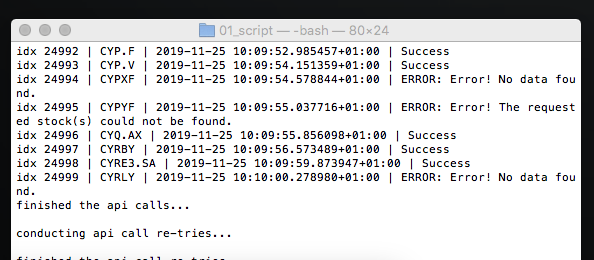
\includegraphics[width=\linewidth]{img/test.png}
		\caption{A boat.}
		\label{fig:boat1}
	\end{figure}
	
	Figure \ref{fig:boat1} shows a boat.
	
	\subsubsection{General}
	
	\subsubsection{Target Variable}
	
	\subsubsection{Feature Variables}
	

	\section{Method}
	
	\subsection{Evaluation Metric}
	
	\subsection{Baseline Models}
	
	\subsection{Advanced Models}
	
	\subsection{Hyperparameter Tuning}
	
	Train vs. test
	
	\subsection{Feature Relevance}
	
	\section{Results}
	
	Table ~\ref{table:prosConsOptionalApproaches} summarizes
	the benefits and drawbacks (``Pros and Cons'') of each 
	approach.
	
	\begin{table}[h]
	\centering
	\caption{The pros and cons of Scala's optional classes}
	\label{table:prosConsOptionalApproaches}
	
	\begin{tabular}{llrrrrr}
		\toprule
		&        & \multicolumn{5}{l}{Predicted} \\
		&        &    lg\_dec & sm\_dec & zero & sm\_inc & lg\_inc \\
		\midrule
		True & lg\_dec &       107 &     46 &   53 &     32 &     78 \\
		& sm\_dec &        39 &     56 &  117 &     49 &     48 \\
		& zero &        34 &     54 &  146 &     46 &     33 \\
		& sm\_inc &        55 &     59 &  102 &     65 &     43 \\
		& lg\_inc &        82 &     42 &   41 &     40 &    128 \\
		\bottomrule
	\end{tabular}
	\end{table}%		

	\section{Discussion}
	
	\section{Conclusion}
	
	\section{References}
	
	
\printbibliography
\end{document}
